\documentclass{article} 
% \usepackage[vietnamese]{babel}
\usepackage[utf8]{vietnam}
\usepackage{graphicx}
\usepackage{biblatex}
\bibliography{references.bib}

\usepackage{dsfont}

\graphicspath{{images/}}


\title{Báo Cáo về Mô Hình CARTE: Tiền Huấn Luyện và Chuyển Giao với Việc Học trên Dữ Liệu Bảng}
\author{Nguyễn Hữu Lộc - 23C15031 \and Lê Trường Vũ - 23C15042}
\date{09/02/2025}

\pagenumbering{arabic}

\begin{document}

\maketitle

\tableofcontents


\section{Giới thiệu sơ lược}
Các mô hình học máy tiền huấn luyện (pre-trained model) hiện nay đã trở nên phổ biến hơn nhiều và góp phần đáng kể vào sự phát triển của lĩnh vực trí tuệ nhân tạo trên nhiều loại dữ liệu khác nhau cả về mặt học thuật lẫn thương mại, nhất là trong các mảng về hình ảnh hay văn bản. Những mô hình này có thể được tải xuống từ các kho lưu trữ như HuggingFace, mang theo một lượng lớn thông tin ngầm và các phép biến đổi phức tạp, giúp tận dụng sức mạnh của học sâu ngay cả khi dữ liệu huấn luyện có quy mô nhỏ. Chính nhờ cách tiếp cận này, các mô hình nền tảng (foundation model), đặc biệt là các mô hình ngôn ngữ lớn (LLM), đã bùng nổ và định hình lại nhiều lĩnh vực.

Tuy nhiên, đối với dữ liệu dạng bảng thì dù loại dữ liệu này có ý nghĩa quan trọng trong môi trường doanh nghiệp và tổ chức nhưng tới hiện tại vẫn chưa có một mô hình nào có thể tạo nền tảng như vậy và trở ngại chính đền từ việc tích hợp dữ liệu từ nhiều bảng khác nhau. Đôi khi, các bảng có thể không chứa bất kỳ thông tin liên quan nào với nhau, và khi có, việc kết nối chúng lại trở thành một bài toán phức tạp trong lĩnh vực nghiên cứu cơ sở dữ liệu. Những thách thức điển hình bao gồm việc tìm mối tương ứng giữa các cột (đối sánh sơ đồ - schema matching) hoặc xử lý các nguồn dữ liệu có cách đặt tên khác nhau cho cùng một đối tượng (đối sánh đối tượng - entity matching). Do sự khác biệt này, việc huấn luyện trước trên dữ liệu bảng vẫn chưa khả thi, khiến phương pháp học sâu chưa thực sự đáng cân nhắc so với các phương pháp khác dựa trên cây quyết định.

Trong nghiên cứu này, nhóm nghiên cứu đã đề xuất kiến trúc học máy CARTE (Context-Aware Representation of Table Entries) có thể học từ nhiều bảng dữ liệu mà không cần phải đối sánh sơ đồ hay đối sánh chuỗi ký tự. Cách tiếp cận cốt lõi của nhóm nghiên cứu là biểu diễn bảng dưới dạng đồ thị, trong đó các cột và giá trị trong bảng được ánh xạ thành các vector nhúng. Mô hình này được huấn luyện trước trên một cơ sở tri thức quy mô lớn, giúp nó có khả năng học hỏi từ một lượng lớn các đối tượng và mối quan hệ. Từ đó, mô hình có thể được tinh chỉnh (fine-tune) để từ đó phục vụ các tác vụ cụ thể, ví dụ như những trường hợp hạn chế về dữ liệu huấn luyện, học từ nhiều bảng cùng lúc hay giúp bổ sung thông tin từ các nguồn dữ liệu thiếu liên kết. Thực nghiệm cho thấy CARTE mang lại sự cải thiện đáng kể về hiệu suất, vượt trội hơn hẳn so với 42 phương pháp cơ sở (baseline), bao gồm cả các phương pháp dựa trên cây quyết định.

\section{Các Nghiên Cứu Liên Quan}
Dữ liệu bảng đóng vai trò quan trọng trong nhiều ứng dụng thực tế, do đó, đã có nhiều phương pháp học sâu được phát triển để xử lý loại dữ liệu này. Tuy nhiên, trong hầu hết các trường hợp, các phương pháp này vẫn chưa thể vượt qua được những mô hình dựa trên cây quyết định. Mặc dù một số nghiên cứu đã chỉ ra rằng mạng nơ-ron có thể hoạt động tốt trên một số loại bảng nhất định nhưng để thực sự tạo vượt qua được thì các mô hình học sâu trên dữ liệu bảng cần phải tạo được một bước ngoặc lớn, chẳng hạn như khả năng tận dụng tri thức nền tảng tương tự như các mô hình ngôn ngữ lớn (LLM) đã làm.

Để tận dụng được dữ liệu lớn để huấn luyện mô hình nền tảng thì học chuyển giao là mấu chốt cần giải quyết. Việc học chuyển giao trong dữ liệu bảng chủ yếu tập trung vào các trường hợp mà tập dữ liệu đích có cùng cấu trúc cột với tập dữ liệu nguồn. Một số phương pháp tiếp cận đã được đề xuất mô hình được huấn luyện trước trên một lượng dữ liệu dạng bảng lớn hơn nhưng không gán nhãn, hoặc sử dụng các bộ dữ liệu liên quan để thu hẹp khoảng cách giữa học sâu và mô hình cây quyết định, đặc biệt là trong bối cảnh dữ liệu y tế. 

Một số phương pháp có thể xử lý các bảng với cột khác nhau bằng cách ánh xạ dữ liệu sang không gian đặc trưng chung, điển hình là XTab, nhưng vẫn chưa đạt hiệu suất tốt hơn so với các mô hình cây hiện đại. Ngoài ra, cũng có các nghiên cứu hướng đến việc biểu diễn từng dòng dữ liệu dưới dạng vector nhúng để học trên nhiều bảng, đặc trưng có Transtab đã vượt qua một số mô hình cơ sở như là XGBoost. Tuy nhiên những phương pháp này có thể mở rộng cho nhiều ứng dụng khác nhau hay không.

Một số tiến bộ đã đạt được trong việc tiền huấn luyện mô hình trên dữ liệu bảng, chẳng hạn như TabPFN – một mô hình Transformer được huấn luyện trên dữ liệu tổng hợp, giúp cải thiện hiệu suất trên các tập dữ liệu nhỏ. Tuy nhiên, nó chưa có cơ chế xử lý tốt các cột dạng phân loại, vốn là một điểm mạnh của các mô hình cây. Các mô hình ngôn ngữ lớn (LLM) cũng đã được thử nghiệm cho dữ liệu bảng, chẳng hạn như TabLLM, trong đó dữ liệu bảng được chuyển thành những chuỗi token để ứng dụng vào việc tinh chỉnh các mô hình LLM. Tuy nhiên, do khó khăn trong việc xử lý dữ liệu số mà mô hình này vẫn chưa có tính cạnh trang. Nhìn chung cả 2 hướng chưa đủ để vượt qua các phương pháp cây. 

Một thách thức quan trọng của dữ liệu bảng là sự xuất hiện của các giá trị rời rạc, thường được biểu diễn dưới dạng chuỗi văn bản. Một số nghiên cứu đã phát triển cách tiếp cận dựa trên biểu diễn chuỗi để hỗ trợ việc học từ loại dữ liệu này. Chẳng hạn như mô hình TableVectorizer chuyển đổi các cột khác nhau thành dạng ma trận số phù hợp cho việc học máy, hoặc mô hình KEN sử dụng phương pháp nhúng trong đồ thị tri thức để mã hóa thông tin từ nguồn như Wikipedia. Tuy nhiên, những phương pháp này thường yêu cầu ánh xạ chính xác từng giá trị của cột sang một thực thể cụ thể liên kết đến Wikipedia, tạo ra nhu cầu phải xử lý thêm tác vụ đối sánh đối tượng (entity matching). 

Các mô hình thống kê truyền thống thường yêu cầu dữ liệu được tập hợp trong một bảng nhất quán, một bài toán thuộc lĩnh vực tích hợp dữ liệu. Một trong những thách thức quan trọng của lĩnh vực này là đối sánh sơ đồ (tìm cột tương ứng giữa các nguồn dữ liệu khác nhau) và đối sánh đối tượng (liên kết các chuỗi ký tự với đối tượng thực tế). Các phương pháp học sâu, đặc biệt là các mô hình dựa trên cơ chế tự chú ý, đã được áp dụng để hỗ trợ chuẩn hóa và tích hợp dữ liệu, giúp tự động hóa nhiều tác vụ mà trước đây cần đến sự can thiệp thủ công. Tuy nhiên, nghiên cứu của nhóm nghiên cứu hướng đến một mục tiêu khác, thay vì dựa vào việc đối sánh rõ ràng các đối tượng hoặc sơ đồ, nhóm nghiên cứu tìm cách khai thác cấu trúc ngầm của dữ liệu để hỗ trợ các bài toán học máy mà không yêu cầu bất kỳ thao tác thủ công nào trong việc tìm kiếm nguồn dữ liệu liên quan. Đây là một vấn đề cấp thiết bởi hiện tại, có nhiều nhóm nghiên cứu đang nỗ lực xây dựng các kho dữ liệu bảng quy mô lớn nhưng do quy mô nhỏ của hầu hết các bảng dữ liệu hiện có và sự khác biệt lớn giữa các tập dữ liệu bảng. 

\section{Cách Mô Hình CARTE Học từ Dữ Liệu Bảng}
CARTE có thể học trên nhiều bảng dữ liệu khác nhau nhờ vào hai yếu tố chính: một cách biểu diễn mới cho đối tượng dạng bảng với cấu trúc đồ thị và một kiến trúc mạng nơ-ron sâu có khả năng nắm bắt ngữ cảnh(context) của bảng. Trong đó, cách biểu diễn đồ thị giúp đồng bộ hóa nhiều bảng dữ liệu vào cùng một không gian biểu diễn, làm cho việc tiền huấn luyện trên các dữ liệu nền tảng thiếu liên kết trước đây trở nên khả thi. Đồng thời, mạng nơ-ron sâu có khả năng nhận thức ngữ cảnh giúp truyền tải các thông tin nền sáng các tác vụ. 

\subsection{Biểu Diễn Đồ Thị của Đối Tượng Bảng} \label{sec:graph_representation}
Việc sử dụng đồ thị là yếu tố quan trọng để giúp khái quát hóa các đối tượng bảng (tabular entity). Một đồ thị $G$ bao gồm tập hợp các nút và cạnh, trong đó các nút biểu diễn đối tượng và các cạnh mô tả quan hệ giữa chúng. Đồ thị là công cụ mạnh mẽ để biểu diễn thông tin quan hệ giữa các đối tượng, và học sâu trên đồ thị đã được chứng minh là có tiềm năng lớn trong các tác vụ liên quan cơ sở dữ liệu có quan hệ (relational database).

CARTE tổ chức mỗi dòng dữ liệu trong bảng dưới dạng một đồ thị nhỏ. Giả sử bảng có $k$ cột, CARTE biểu diễn dòng dữ liệu thứ $i$ dưới dạng một đồ thị $G_i(X,E)$ trong đó $X$ và $E$ lần lượt là đặc trưng của nút và cạnh. Cấu trúc của $G_i(X,E)$ có dạng một đồ thị hình sao với $k$ nút lá trừ đi $p_i$ nút với $p_i$ là số cột có giá trị bị thiếu trong dòng $i$. Trên mỗi đồ thị con này, các nút lá được gán nhãn theo giá trị ô dữ liệu và tên cột tương ứng, có thể thấy thông qua Hình \ref{fig:graphlet_representation_of_tabular_entity}.

Để biến đồ thị này thành đầu vào cho mạng nơ-ron, CARTE sử dụng một mô hình ngôn ngữ để khởi tạo các đặc trưng. Cụ thể là với các giá trị phân loại và tên cột, CARTE dùng mô hình ngôn ngữ để chuyển đổi giá trị thành dữ liệu dạng nhúng có $d$ chiều. Với các giá trị số, đặc trưng của nút được khởi tạo bằng cách nhân giá trị số với nhúng của tên cột tương ứng. Ví dụ như ở Hình \ref{fig:graphlet_representation_of_tabular_entity}, nếu một ô chứa giá trị 239 trong cột "H index", đặc trưng của nút đó sẽ là $239 \times E_{H index}$. Nút trung tâm của đồ thị được khởi tạo bằng giá trị trung bình của các nút lá và sẽ đóng vai trò là nút "readout". Trong mạng Neural Graph (Graph Neural Network - GNN), nút "readout" (nút đọc) là một quá trình tổng hợp thông tin từ các nút của đồ thị để tạo ra một biểu diễn đặc trưng có ý nghĩa cho toàn bộ đồ thị hoặc một phần của nó. 

\begin{figure} 
    \centering
    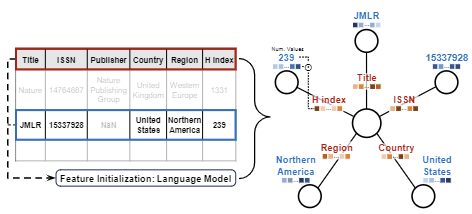
\includegraphics[scale = 1]{graphlet_representation_of_tabular_entity.png}
    \caption{CARTE biểu diễn mỗi hàng của bảng dưới dạng một đồ thị nh(graphlet). Các nút lá chứa giá trị ô và tên cột tương ứng và các đặc trưng nút được khởi tạo thông qua mô hình ngôn ngữ.}
    \label{fig:graphlet_representation_of_tabular_entity}
\end{figure}

Ưu điểm của cách biểu diễn đồ thị là cách tiếp cận này mang lại nhiều lợi ích. Giữ ngữ cảnh của dữ liệu bảng: Trong dữ liệu bảng, mỗi giá trị chỉ có ý nghĩa khi được xem xét trong ngữ cảnh của tên cột. Ví dụ như ở Hình \ref{fig:graphlet_representation_of_tabular_entity}, một dòng dữ liệu gồm các giá trị "JMLR", "15337928", "239" sẽ khó hiểu nếu không có tên cột đi kèm. Tuy nhiên, khi biết rằng chúng thuộc các cột "Title", "ISSN" và "H index", ta có thể nhận ra rằng đây là một tạp chí học thuật và CARTE khai thác ngữ cảnh này thông qua sự liên kết trong cấu trúc đồ thị từ đó phục vụ việc học cấu trúc của dữ liệu.

Vì các bảng có thể có số lượng cột khác nhau hoặc trật tự cột khác nhau, cách biểu diễn đồ thị của CARTE giúp kết nối dữ liệu mà không cần phải dữ liệu tên cột. Điều này mở ra khả năng học trên nhiều bảng mà không cần đối sánh sơ đồ. Bên cạnh đó, việc CARTE sử dụng mô hình ngôn ngữ để xử lý các giá trị dạng văn bản, danh mục và tên cột, giúp giảm bớt công đoạn tiền xử lý dữ liệu như mã hóa phân loại hay loại bỏ trùng lặp. Ngoài ra, CARTE có thể xử lý các từ vựng mở rộng, cho phép nhận diện những biến thể ngôn ngữ như "North America" và "Northern America" mà không cần các tác vụ gán ghép thủ công.

Nhờ những đặc điểm trên, cách tiếp cận đồ thị của CARTE giúp khái quát hóa dữ liệu từ các bảng không đồng nhất, đưa tất cả các bảng vào cùng một miền biểu diễn mà không cần phải thực hiện đối sánh sơ đồ hay đối sánh đối tượng. Điều này tạo điều kiện cho việc học trên nhiều bảng, mở ra cơ hội tiền huấn luyện và học chuyển giao trên dữ liệu bảng một cách hiệu quả.


\subsection{Tiền Huấn Luyện Mô Hình từ Cơ Sở Tri Thức Lớn}

\begin{figure} 
    \centering
    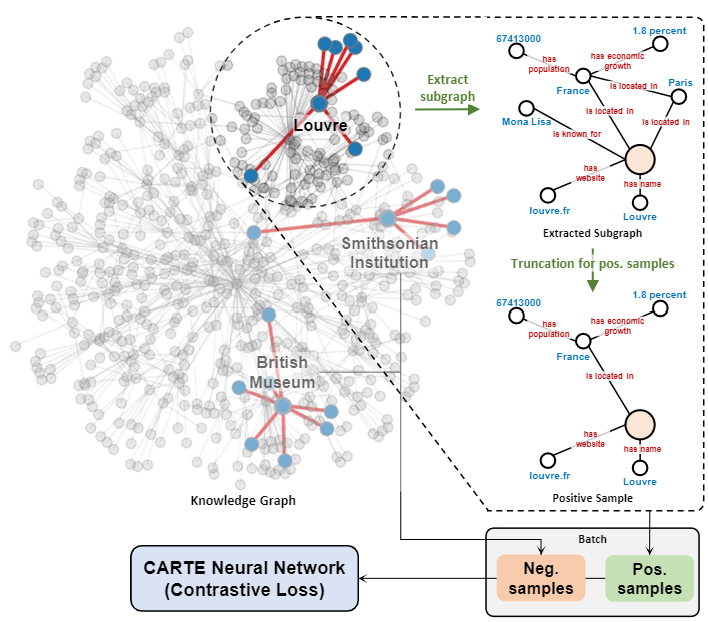
\includegraphics[scale = 0.8]{carte_pretraining_process.png}
    \caption{CARTE tiền huấn luyện bằng cách tạo graphlet từ một đồ thị tri thức lớn. Những graphlet này được đưa vào mạng nơ-ron để huấn luyện theo phương pháp tự giám sát, giúp mô hình học cách tổng hợp thông tin từ các bảng thông qua quan hệ giữa các cột.}
    \label{fig:carte_pretraining_process}
\end{figure}

CARTE được tiền huấn luyện trên YAGO3, một cơ sở tri thức lớn được xây dựng từ Wikidata và các nguồn khác, chứa thông tin thực tế về thế giới. YAGO lưu trữ dữ liệu dưới dạng đồ thị tri thức, bao gồm các bộ ba (head, relation, tail). Ví dụ, bộ ba (“Louvre”, “is located in”, “Paris”) trong Hình \ref{fig:carte_pretraining_process} là một mẫu dữ liệu có thể tìm thấy trong YAGO. Phiên bản hiện tại của YAGO chứa hơn 18,1 triệu bộ ba với 6,3 triệu thực thể.

Trong phần này, nhóm sẽ mô tả quá trình tiền huấn luyện của mô hình CARTE, được tóm tắt trong Hình \ref{fig:carte_pretraining_process}. Từ đồ thị tri thức, các đồ thị con (graphlets) phù hợp sẽ được trích xuất để xử lý làm đầu vào cho CARTE. Để thực hiện học tự giám sát với hàm mất mát tương phản (contrastive loss), nhóm thêm vào batch các phiên bản bị cắt ngắn của các graphlets đã chọn để đó mô hình học cách tổng hợp thông tin dựa trên ngữ cảnh được cung cấp.

Từ đồ thị tri thức lớn YAGO, các graphlet nhỏ hơn được tạo nên giới hạn các liên kết trong phạm vi $k$ quan hệ liên kết (k-hop relations). Để duy trì cấu trúc được trình bày trong Hình \ref{fig:graphlet_representation_of_tabular_entity}, đồng thời tận dụng thêm thông tin từ nhiều bước nhảy, k=2 đã được lựa chọn kết hợp với giới hạn số lượng quan hệ 1-hop và 2-hop lần lượt là 100 và 10.

Các graphlets từ bảng dữ liệu trong Hình \ref{fig:graphlet_representation_of_tabular_entity} sử dụng một token làm node trung tâm (center node) cho mỗi hàng, trong khi các graphlets từ đồ thị tri thức có thể sử dụng tên thực thể (ví dụ: "Louvre"). Để tránh sự khác biệt này, nhóm sử dụng một token làm node trung tâm, kèm theo một node bổ sung chứa tên thực thể và được kết nối bằng quan hệ "has name". Cuối cùng, tương tự như đã đề cập ở phần \ref{sec:graph_representation}, nhóm khởi tạo các node và cạnh bằng cách sử dụng embedding từ mô hình ngôn ngữ FastText.

Để tạo một batch mẫu với kích thước $N_b$, đầu tiên nhóm chọn các thực thể từ YAGO sẽ được đưa vào batch và tạo các graphlets tương ứng. Trong đó, 90\% $N_b$ được lấy từ các thực thể có ít nhất 6 quan hệ 1-hop, 10\% còn lại được lấy từ các thực thể khác. Lý do chính cho việc lấy mẫu như vậy là do phần lớn thực thể trong YAGO chỉ có một hoặc hai quan hệ 1-hop, trong khi dữ liệu dạng bảng thường có nhiều hơn (tương ứng với nhiều cột).

Để áp dụng học tự giám sát với mất mát tương phản, nhóm tạo ra các mẫu dương bằng cách rút gọn cấu trúc thông qua việc xóa một phần ngẫu nhiên (từ 30\% đến 70\%) số cạnh trong graphlets gốc. Hình \ref{fig:carte_pretraining_process} minh họa một graphlet của thực thể "Louvre" cùng với phiên bản bị cắt ngắn của nó.

\begin{figure} 
    \centering
    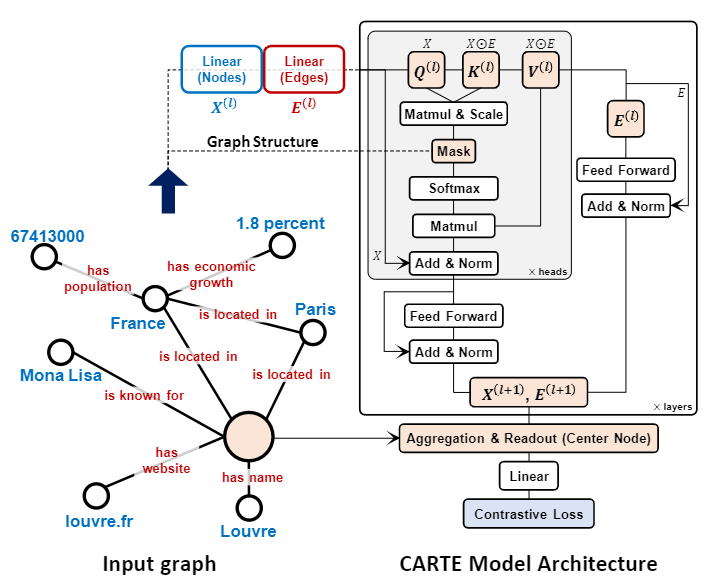
\includegraphics[scale = 0.8]{carte_architecture.png}
    \caption{CARTE sử dụng các đồ thị làm đầu vào, với đặc trưng là các nút và cạnh được dùng trong huấn luyện lớp self-attention. Các lớp này cập nhật đặc trưng nút dựa trên thông tin cạnh và sử dụng attention mask để duy trì cấu trúc đồ thị. Lớp Tổng hợp \& Đọc trích xuất đặc trưng từ nút trung tâm (center node), và đầu ra cuối cùng được dùng để tính toán cho hàm mất mát đối lập (contrastive loss).}
    \label{fig:carte_architecture}
\end{figure}

Hình \ref{fig:carte_architecture} mô tả kiến trúc của CARTE. Về cơ bản, CARTE sử dụng mô hình Transformer encoder truyền thống của và sửa đội thành một mạng đồ thị với cơ chế chú ý (graph attentional network). Một thành phần quan trọng trong kiến trúc của CARTE là lớp tự chú ý (self-attention) tính toán mức độ quan trọng của các node và cạnh trong đồ thị. Trong mô hình đồ thị, cơ chế chú ý điều chỉnh tầm quan trọng của các node lân cận đối với một node nhất định. Đối với dữ liệu bảng, điều này có nghĩa là xác định mức độ quan trọng của từng giá trị trong hàng, với ngữ cảnh được bổ sung bởi thông tin cột.

Đi sâu vào thì cơ chế tập trung (attention) của CARTE được thiết kế để nắm bắt ngữ cảnh và mối quan hệ giữa các thành phần. Có ba thành phần chính cần chú ý là truy vấn (query), khóa (key), và giá trị (value), trong đó truy vấn đại diện cho thông tin cần quan tâm—trong trường hợp này là các nút. Vì vậy, chúng ta sử dụng cách tiếp cận phổ biến và chỉ dựa vào thông tin của nút để xây dựng truy vấn. Ngược lại, cặp khóa-giá trị cần phản ánh những thông tin mà các nút lân cận có thể cung cấp. Do đó, ta đưa thông tin cạnh vào quá trình xây dựng khóa và giá trị. Cụ thể, ba thành phần này được xác định như Hình \ref{fig:architecture_attention_mechanic}.

\begin{figure} 
    \centering
    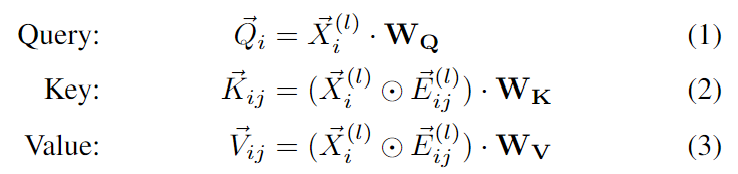
\includegraphics[scale = 0.8]{architecture_attention_mechanic.png}
    \caption{3 thành phần chính của cơ chế attention}
    \label{fig:architecture_attention_mechanic}
\end{figure}

Các yếu tố $W_Q, W_K, W_V$ như trong Hình \ref{fig:architecture_attention_mechanic} là các trọng số để huấn luyện và dấu $\odot$ đánh dấu phép nhân từng phần tử (element-wise multiplication) được lấy cảm hứng từ một số nghiên cứu khác về phương pháp nhúng đồ thị tri thức. Dựa trên công thức tính attention score theo phương pháp scaled dot-product attention, trọng số tập trung của nút $j$ với nút $i$, ký hiệu là $A_ij$ được tính như Hình \ref{fig:attention_score}. 

\begin{figure} 
    \centering
    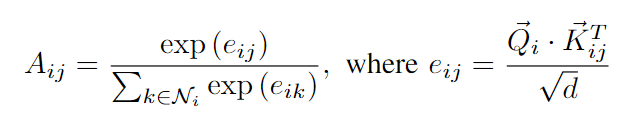
\includegraphics[scale = 0.8]{attention_score.png}
    \caption{Công thức Attention Score theo phương pháp scaled dot-product attention}
    \label{fig:attention_score}
\end{figure}

Ở đây, tổng chỉ xét trên các nút lân cận của $i$, điều này tương ứng với bước "che mặt nạ" (masking) để bảo toàn cấu trúc đồ thị. Việc đưa loại quan hệ (như nhãn cột trong bảng dữ liệu) vào tính toán attention giúp mô hình tái diễn giải ngữ cảnh chính xác hơn. Chẳng hạn, một thực thể như "George Bush" có thể chỉ tổng thống thứ 41 hoặc 43 của Mỹ, hoặc một tàu sân bay mang tên này. Ý nghĩa của nó phụ thuộc vào mối quan hệ đi kèm (ví dụ: "George Bush", "con của", "George Bush"). Nếu thay bằng mối quan hệ khác như "cha của", thì cách xác định thực thể sẽ thay đổi hoàn toàn.

Đầu ra của các lớp attention được biểu diễn thông qua các đặc trưng đã được biến đổi của nút và cạnh. Ở các tầng cuối cùng, mô hình sử dụng một lớp attention nhưng không cập nhật thông tin cạnh. Sau đó, một lớp tổng hợp (readout layer) sẽ trích xuất biểu diễn của nút trung tâm. Đối với giai đoạn tiền huấn luyện (pretraining), đầu ra từ mô hình sẽ được xử lý để tính toán hàm mất mát tương phản (contrastive loss) như trong Hình \ref{fig:carte_pretraining_process}. 


\subsection{Tinh Chỉnh cho Tác Vụ}
Trong một tác vụ đầu ra cụ thể, quá trình tinh chỉnh CARTE chỉ sử dụng lại một phần của kiến trúc đã được huấn luyện trước (như minh họa trong Hình \ref{fig:carte_architecture}). Cụ thể, các lớp ban đầu xử lý nút và cạnh (khối màu xanh và đỏ trong Hình \ref{fig:carte_architecture}) cùng với lớp "Tổng hợp \& Đọc ra" được giữ lại.

Thực tế, các thực thể trong bảng đầu ra có cấu trúc đồ thị đơn giản hơn so với giai đoạn huấn luyện ban đầu. Thứ nhất, chúng thường có dạng hình sao (Hình \ref{fig:graphlet_representation_of_tabular_entity}). Thứ hai, các bảng đầu ra có ít sự biến đổi về cấu trúc đồ thị hơn và số lượng biến rời rạc cũng thấp hơn so với dữ liệu ban đầu từ YAGO. Nếu kiến trúc quá sâu, các đặc trưng phân biệt có thể bị làm mờ trong biểu diễn đầu ra, dẫn đến hiện tượng làm mịn quá mức. Do đó, nhóm đã áp dụng một quy ước phổ biến trong mô hình đồ thị là số lớp attention sẽ tương đương với số bậc quan hệ tối đa, trong trường hợp này là $k=1$. Đối với phân lớp cuối cùng, các lớp tuyến tính được gắn trực tiếp vào mô hình. Khi tinh chỉnh mô hình cơ sở, hai phương thức suy luận khác nhau sẽ được xem xét với chi tiết trong phần sau.

\subsubsection{Suy luận trên dữ liệu bảng đơn}
Đây là kịch bản phổ biến, trong đó một bảng duy nhất được cung cấp với biến mục tiêu cần dự đoán. Trước khi chuyển đổi các thực thể bảng thành đồ thị, nhóm áp dụng biến đổi lũy thừa (power transform) lên các biến giá trị số nhằm cải thiện độ ổn định của mô hình. Biến đổi này đã được chứng minh hiệu quả trong nhiều nghiên cứu trước đây và giúp quá trình tinh chỉnh CARTE ổn định hơn. Ngoài ra, nhóm áp dụng chiến lược bagging, hay còn gọi là boostrap aggregating, trong đó nhiều mô hình được huấn luyện song song với các tập dữ liệu khác nhau được chia nhỏ theo chiến lược. Kết quả dự đoán cuối cùng được tính bằng cách lấy trung bình đầu ra của các mô hình này.

\subsubsection{Học chuyển giao từ một bảng nguồn sang bảng đích}
Nhóm cũng sử dụng CARTE trong các bài toán học chuyển giao, nơi có một bảng nguồn $X_S$ có thể hỗ trợ dự đoán trên bảng đích $X_T$. Đáng chú ý, bảng nguồn thường có số lượng mẫu huấn luyện lớn hơn so với bảng đích và việc tinh chỉnh mô hình cần được thực hiện đồng thời trên cả hai bảng. Nhờ vào biểu diễn đồ thị, mô hình có thể tinh chỉnh đồng thời mà không cần sự tương ứng giữa các cột của hai bảng nhưng kết quả đầu ra $y_S$ và $y_T$ của bảng nguồn $X_S$ và bảng đích $X_T$ cần phải tương đồng.

Để đảm bảo điều này, nhóm thực hiện một bước chuyển đổi trên $y_S$ để phù hợp với kỳ vọng toán học bậc nhất của $y_T$ bằng cách sử dụng phép biến đổi lũy thừa như trước đó, nhưng lần này áp dụng phép biến đổi nghịch đảo. Nếu bản chất của biến mục tiêu giữa bảng nguồn và bảng đích khác nhau (phân loại hoặc hồi quy), nhóm điều chỉnh $y_S$ như sau:

\begin{itemize}
    \item Nếu $y_T$ thuộc tác vụ phân loại, nhóm sẽ nhị phân hóa biến hồi quy trọng bảng nguồn $X_S$.
    \item Nếu $y_T$ là thuộc tác vụ hồi quy, nhóm sẽ sử dụng biến phân loại của bảng nguồn $X_S$, mã hóa nó dưới dạng {0,1} và chuẩn hóa theo phương pháp chuẩn.
\end{itemize}

Quá trình tinh chỉnh CARTE tiếp tục bằng cách lấy các tập dữ liệu với tỷ lệ cố định các dòng từ bảng nguồn và bảng đích (trong đó mỗi tập có kích thước 64, với 8 dòng trong đó đến từ bảng đích). Chiến lược dừng sớm được thực hiện trên tập xác thực của bảng đích, và dựa phương pháp bagging để tạo ra nhiều mô hình con huấn luyện trên các tập xác thực khác nhau và kết quả dự đoán là trung bình kết quả tổng hợp lại của các mô hình con.

Thông thường thì quá trình dừng sớm diễn ra trước khi tất cả các điểm dữ liệu của bảng nguồn được sử dụng. Điều này giúp tránh hiện tượng overfitting vào dữ liệu nguồn, vì dữ liệu nguồn có thể không quan trọng bằng dữ liệu đích đối với việc dự đoán $y_T$. Các siêu tham số được sử dụng vẫn giữ nguyên như trong thiết lập với một bảng đơn lẻ.

Vì nhóm đã chọn bảng nguồn khá linh hoạt từ dữ liệu có liên quan yếu, nên không phải lúc nào mô hình học theo cặp (pairwise learner) cũng cải thiện so với mô hình học trên một bảng đơn lẻ, đặc biệt khi bảng nguồn không cung cấp đủ thông tin liên quan. Để khắc phục, nhóm kết hợp mô hình học theo cặp với mô hình học đơn lẻ bằng cách tổng hợp (ensemble) dự đoán của cả hai cách thông qua hàm softmax. Trọng số trong softmax được xác định dựa trên điểm dự đoán từ tập xác thực nội bộ của các mô hình thành phần. Để điều chỉnh nhiệt độ (temperature) của softmax, trọng số sẽ được chia cho độ lệch chuẩn (standard deviation) giữa các mô hình, giúp cân bằng ảnh hưởng của từng mô hình trong tổ hợp.

\subsubsection{Học chung trên nhiều bảng}
Mấu chốt của học chuyển giao, như đã đề cập ở trên, là cần phải tìm được bảng nguồn phù hợp. Nếu có nhiều bảng từ cùng một lĩnh vực, CARTE có thể tận dụng tất cả để chọn lọc thông tin hữu ích nhất cho tác vụ học chuyển giao. Trong trường hợp này, bài toán được đặt ra với một bảng đích $X_T$ và một tập hợp các bảng nguồn \{$X_{S,1}, ..., X_{S,m}$\}. Quá trình huấn luyện như sau:
\begin{enumerate}
    \item Xây dựng mô hình học đơn lẻ trên $X_T$.
    \item Xây dựng từng mô hình học cặp giữa bảng đích $X_T$ và từng bảng nguồn $X_{S,i}$ bằng phương pháp học cặp đã mô tả ở trên.
    \item Kết hợp (ensemble) các mô hình học cặp cùng với mô hình học đơn lẻ
\end{enumerate}

Không phải mọi cặp bảng đều mang lại thông tin hữu ích như nhau nên để tìm tổ hợp dữ liệu tối ưu thì phần Ensemble là cần thiết. Nếu tất cả các bảng nguồn đều tạo ra dự đoán tốt, chúng sẽ được kết hợp với trọng số bằng nhau, nhưng nếu một bảng nguồn vượt trội hơn, kết quả dự đoán sẽ được neo vào bảng đó.

\section{Nghiên Cứu Thực Nghiệm}
\subsection{Cài Đặt Thực Nghiệm}
Trong nghiên cứu này nhóm đã sử dụng 51 tập dữ liệu dạng bảng, trong đó có 40 tập dành cho bài toán hồi quy và 11 tập dành cho bài toán phân loại. Các tập dữ liệu này được thu thập từ nhiều nguồn khác nhau, chủ yếu từ các nghiên cứu trước đây về học máy và các cuộc thi trên Kaggle gồm nhiều chủ đề liên quan đến xã hội và kinh doanh, chẳng hạn như tai nạn, bầu cử, tiền lương, thực phẩm, nhà hàng, ... Các tập dữ liệu được chọn có thể nói là đại diện cho các ứng dụng khoa học dữ liệu hiện đại, với các bảng có cột có ý nghĩa và các giá trị rời rạc.

Trong bài báo, nhóm nghiên cứu đánh giá và so sánh với nhiều phương pháp cơ sở khác nhau, chi tiết như danh sách sau: 

\begin{itemize}
    \item CatBoost: Một thuật toán cây tăng cường độ dốc (gradient boosting) phổ biến để học trên dữ liệu dạng bảng. Các đặc trưng dạng văn bản được xử lý dưới dạng dữ liệu phân loại, mã hóa bằng phương pháp mã hóa mục tiêu.
    \item TabVec: Sử dụng bộ TableVectorizer từ thư viện Skrub để mã hóa các bảng có dữ liệu dạng chuỗi thành mảng số. Các cột có ít giá trị phân loại được mã hóa one-hot, trong khi các cột có nhiều giá trị phân loại được mã hóa bằng bộ mã hóa Gamma-Poisson. Với các mô hình không dựa trên cây, các giá trị bị thiếu được thay thế bằng giá trị trung bình nếu là đặc trưng số, và được coi là một nhóm riêng đối với đặc trưng phân loại. Với mô hình mạng nơ-ron, dữ liệu được chuẩn hóa về khoảng [0, 1] bằng phương pháp min-max.
    \item XGB, HGB, RF: Các mô hình cây quyết định.
    \item MLP và ResNet: Mạng nơ-ron đa tầng (MLP) và phiên bản mở rộng của nó.
    \item Ridge và Logistic: Các mô hình tuyến tính, bao gồm hồi quy Ridge và hồi quy Logistic.
    \item S-LLM: Dựa trên ý tưởng từ TabLLM, thử nghiệm cách mã hóa từng hàng dữ liệu bằng một mô hình ngôn ngữ lớn (LLM) với mỗi hàng được biểu diễn dưới dạng một câu và mã hóa bằng mô hình intfloat/e5-small-v2 từ HuggingFace. Khác với TabLLM, đầu ra được chuyển vào mô hình XGB để học cho cả hai bài toán hồi quy và phân loại. 
    \item TabPFN: Mô hình transformer huấn luyện trước trên dữ liệu tổng hợp (synthetic) với các đặc trưng văn bản được xử lý dưới dạng phân loại và mã hóa với phương pháp mã hóa mục tiêu.
\end{itemize}


\subsection{Kết Quả trên Bảng Đơn} 
Trong mảng học trên bảng dữ liệu đơn thì CARTE vượt trội so với các phương pháp khác. Hình \ref{fig:carte_performance_comparison} so sánh hiệu suất trong tác vụ dự đoán trên các bộ dữ liệu khác nhau và kết quả cho thấy CARTE luôn đạt hiệu suất cao hơn so với các phương pháp thay thế, bất kể kích thước mẫu.

\begin{figure} 
    \centering
    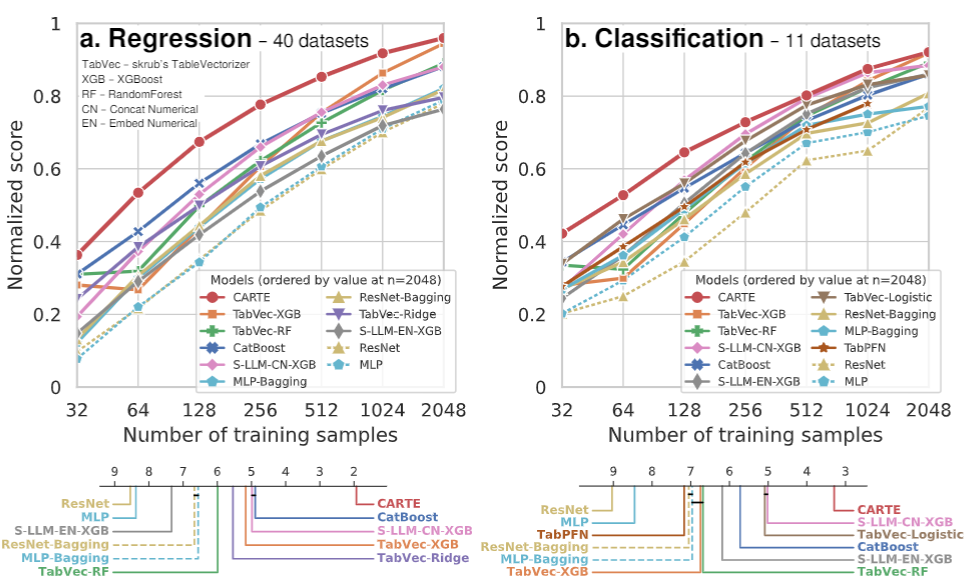
\includegraphics[scale = 0.7]{carte_performance_comparison.png}
    \caption{CARTE đạt hiệu suất tốt nhất khi học trên các bảng đơn lẻ, được đánh giá qua các bài toán hồi quy và phân loại. Điểm số chuẩn hóa cho thấy CARTE vượt trội so với các phương pháp khác trên nhiều kích thước tập huấn luyện. Sơ đồ khác biệt tới hạn minh họa sự chênh lệch hiệu suất giữa các mô hình trên toàn bộ tập dữ liệu.}
    \label{fig:carte_performance_comparison}
\end{figure}

Một điểm quan trọng là chiến lược bagging mà CARTE sử dụng có tác động tích cực đến các mô hình mạng nơ-ron. Việc áp dụng bagging với các tập huấn luyện/kiểm định khác nhau để dừng sớm có thể mang lại lợi ích cho học sâu nói chung.

\begin{figure} 
    \centering
    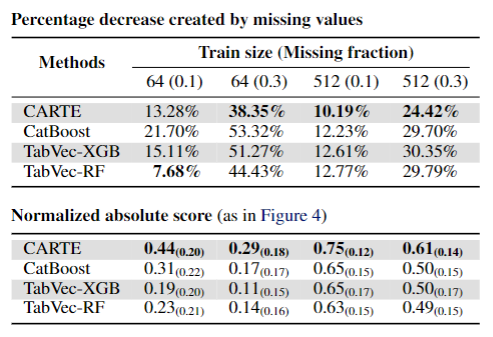
\includegraphics[scale = 0.8]{carte_robust_to_missing_value.png}
    \caption{CARTE cho thấy độ ổn định cao khi xử lý dữ liệu thiếu. Hiệu suất chỉ giảm nhẹ khi một tỷ lệ đặc trưng (10\% hoặc 30\%) bị loại bỏ ngẫu nhiên. Điểm số chuẩn hóa phản ánh khả năng thích ứng tốt của mô hình với dữ liệu không đầy đủ.}
    \label{fig:carte_robust_to_missing_value}
\end{figure}

Khi gặp giá trị bị thiếu, CARTE loại bỏ các cột có dữ liệu thiếu trong bước xây dựng đồ thị. Ví dụ, nếu một điểm dữ liệu có một giá trị bị thiếu trong bảng gồm 10 cột, thì sau khi xây dựng đồ thị, điểm đó sẽ có chín nút lá. Hình \ref{fig:carte_robust_to_missing_value} so sánh mức độ suy giảm hiệu suất (tính theo phần trăm) và điểm số chuẩn hóa (so với Hình \ref{fig:carte_performance_comparison}) giữa CARTE và một số mô hình cây quyết định có khả năng xử lý dữ liệu thiếu. Trong thí nghiệm thì nhóm đã ngẫu nhiên loại bỏ một số đặc trưng của từng mẫu (bao gồm cả tập huấn luyện và kiểm tra) với tỷ lệ 10\% và 30\% và kết quả cho thấy CARTE vẫn duy trì hiệu suất vượt trội so với các mô hình cơ sở khác.

\begin{figure} 
    \centering
    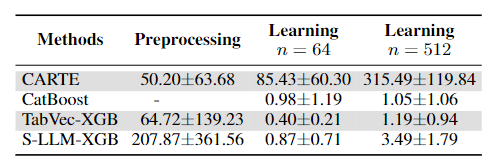
\includegraphics[scale = 0.8]{carte_computation_time.png}
    \caption{Thời gian tính toán (đơn vị giây) được đo lường cho bốn phương pháp hàng đầu, bao gồm các giai đoạn tiền xử lý, huấn luyện và kiểm tra trên 51 tập dữ liệu. So sánh này giúp đánh giá hiệu suất tổng thể của các mô hình trong thực tế.}
    \label{fig:carte_computation_time}
\end{figure}

Bảng \ref{fig:carte_computation_time} thể hiện thời gian tính toán trung bình (tính bằng giây) của bốn mô hình hàng đầu. Hiệu suất dự đoán mạnh mẽ của CARTE đi kèm với chi phí tính toán cao hơn, và sự khác biệt này càng lớn khi kích thước tập huấn luyện tăng lên. Điều này cho thấy cần có những tối ưu hóa bổ sung để giảm chi phí tính toán.

Một giả thuyết giải thích hiệu suất cao của CARTE là mô hình này đã tích hợp thông tin từ nhiều đối tượng nhờ được huấn luyện trước trên cơ sở tri thức YAGO. Tuy nhiên, trong một bảng dữ liệu cụ thể, cách viết tên đối tượng có thể khác nhau, chẳng hạn "Londres" thay vì "London". Điều này đặt ra câu hỏi liệu CARTE có thể chuyển giao thông tin một cách hiệu quả khi cách biểu diễn chuỗi của đối tượng thay đổi hay không. Trong một số trường hợp, đối sánh chuỗi là cần thiết, chẳng hạn khi sử dụng các nhúng véc-tơ của đối tượng như KEN embeddings.

\begin{figure} 
    \centering
    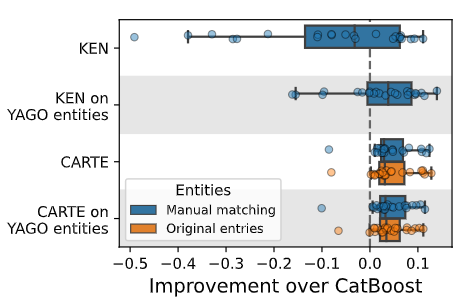
\includegraphics[scale = 0.8]{carte_entity_matching_not_required.png}
    \caption{CARTE không yêu cầu đối sánh thực thể, và các thực thể trong bài toán không cần xuất hiện trong YAGO. Nhóm đánh giá CARTE và KEN trên toàn bộ tập dữ liệu cũng như phiên bản rút gọn chỉ chứa các thực thể có trong YAGO. Khi sử dụng KEN để bổ sung thông tin, CatBoost được chọn làm bộ ước lượng, với các thực thể không khớp bị thay thế bằng giá trị thiếu. Kết quả cho thấy KEN giúp cải thiện hiệu suất của CatBoost trên các thực thể trong YAGO, xác nhận giá trị của việc bổ sung từ thông tin nền.}
    \label{fig:carte_entity_matching_not_required}
\end{figure}

Nhóm đã thực hiện đối sánh thực thể thủ công trên bốn bộ dữ liệu: "company employees", "movies", "US accidents", và "US election". Các thực thể trong dữ liệu này được liên kết với thực thể tương ứng trong cơ sở tri thức YAGO. Hình \ref{fig:carte_entity_matching_not_required} cho thấy rằng trong khi KEN yêu cầu đối sánh thực thể để đạt hiệu suất tốt, CARTE vẫn duy trì độ chính xác cao nhờ vào mô hình hóa ở cấp độ chuỗi. Điều này giúp CARTE trở nên linh hoạt hơn khi xử lý các biến thể khác nhau của thực thể, bất kể sử dụng thực thể đã được đối sánh thủ công hay dữ liệu gốc ban đầu. 

\begin{figure} 
    \centering
    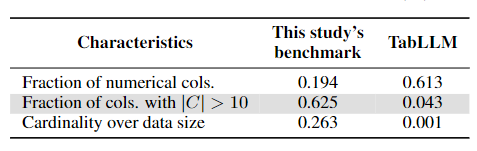
\includegraphics[scale = 0.8]{carte_vs_tabllm_dataset.png}
    \caption{Bộ dữ liệu đánh giá trong nghiên cứu này khác với bộ dữ liệu của TabLLM ở chỗ chứa nhiều cột danh mục hơn, đặc biệt là các cột có số lượng giá trị phân biệt (cardinality) cao. Điều này giúp kiểm tra khả năng xử lý dữ liệu bảng phức tạp của các mô hình một cách toàn diện hơn.}
    \label{fig:carte_vs_tabllm_dataset}
\end{figure}

\begin{figure} 
    \centering
    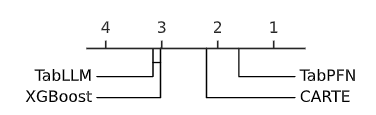
\includegraphics[scale = 0.8]{carte_baseline_comparision.png}
    \caption{So sánh với ba phương pháp trong TabLLM cho thấy rằng các tập dữ liệu này chủ yếu chứa đặc trưng số hoặc cột danh mục có số lượng giá trị thấp. Trong bối cảnh này, TabPFN đạt hiệu suất cao nhất, tiếp theo là CARTE, XGBoost và cuối cùng là TabLLM.}
    \label{fig:carte_baseline_comparision}
\end{figure}

Nhóm nghiên cứu đã so sánh CARTE với ba mô hình cơ sở trên chín bộ dữ liệu thuộc TabLLM. So với các bộ dữ liệu trong Hình \ref{fig:carte_performance_comparison}, tập dữ liệu của TabLLM có tỷ lệ hiệu quả cao hơn các đặc trưng dạng số và ít đặc trưng phân loại có nhiều giá trị (xem Hình \ref{fig:carte_vs_tabllm_dataset}). Hình \ref{fig:carte_baseline_comparision} thể hiện sơ đồ sự khác biệt có ý nghĩa thống kê giữa các mô hình. Trong những điều kiện này, TabPFN cho thấy hiệu suất mạnh mẽ. Tuy nhiên, dù được thiết kế để xử lý cả dữ liệu dạng số và chuỗi, CARTE vẫn đạt được kết quả cạnh tranh.

\subsection{Học Đa Bảng}
Nhóm đã nghiên cứu khả năng học trên nhiều bảng dữ liệu mà không có sự tương quang rõ ràng giữa các cột. Các bảng này được lấy từ nhiều nguồn khác nhau không có cấu trúc đồng nhất nhưng phản ánh cùng một chủ đề tổng quát, như giá xe đạp, đánh giá nhà hàng. Trong bộ dữ liệu gồm 51 bảng, nhóm đã xác định các bộ có nội dung tương tự dù đến từ các nguồn khác nhau.

Trong bối cảnh này, CARTE và S-LLM có thể được sử dụng trực tiếp, vì cả hai đều sử dụng biểu diễn từ vựng mở để ánh xạ các mục nhập vào không gian nhúng. Tuy nhiên, chỉ phiên bản EN (Embed Numerical) của S-LLM mới hoạt động tốt, trong khi phiên bản CN (Concat Numerical) yêu cầu sự tương ứng giữa các cột số.

Với CatBoost, do có khả năng xử lý dữ liệu thiếu một cách tự nhiên, nhóm đã thử nghiệm bằng cách ghép nối các tập dữ liệu và điền giá trị thiếu vào các cột không khớp. Ngoài ra, nhóm cũng kiểm tra hiệu quả của việc đối sánh cột thủ công.

\begin{figure} 
    \centering
    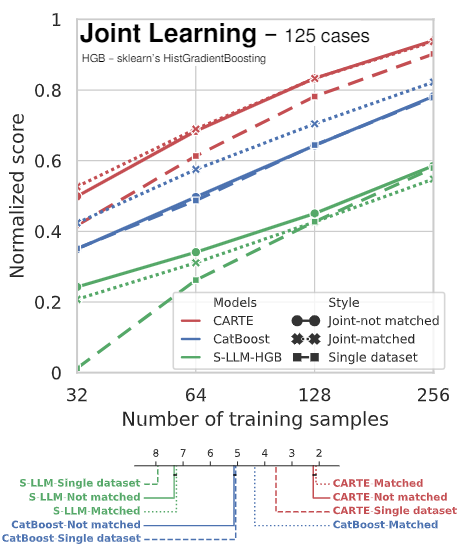
\includegraphics[scale = 0.7]{carte_schema_matching_not_required.png}
    \caption{CARTE không yêu cầu đối sánh lược đồ và vẫn cải thiện hiệu suất nhờ học chung. Nhóm so sánh ba kịch bản: học trên bảng đơn lẻ (đường nét đứt), học chuyển giao tự động không cần thao tác thủ công (đường liền), và học chuyển giao sau khi đối sánh cột thủ công (đường chấm). Kết quả cho thấy học chung giúp CARTE đạt hiệu suất cao một cách nhất quán.}
    \label{fig:carte_schema_matching_not_required}
\end{figure}

Hình \ref{fig:carte_schema_matching_not_required} trình bày kết quả của việc học chuyển giao giữa hai bảng dữ liệu và kết quả là tất cả phương pháp đều có lợi từ học chuyển giao (đường đứt nét, đại diện cho việc học chỉ trên bảng mục tiêu, luôn có hiệu suất thấp hơn). Tuy nhiên, chỉ có CARTE mang lại cải thiện ổn định mà không cần đối sánh cột thủ công.

Đối với CatBoost, việc đối sánh cột (đường chấm) đóng vai trò quan trọng, trong khi với các phương pháp khác thì không. Đối với S-LLM, lợi ích của học chuyển giao giảm nhanh khi số lượng mẫu huấn luyện tăng lên. Nhìn chung, CARTE có thể học từ nhiều bảng khác nhau mà không cần đối sánh lược đồ, đồng thời vẫn mang lại hiệu suất ổn định trên bảng mục tiêu.

\begin{figure} 
    \centering
    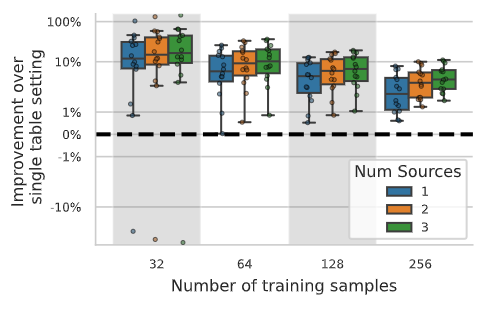
\includegraphics[scale = 0.8]{carte_benefits_from_additional_source_tables.png}
    \caption{CARTE tiếp tục cải thiện hiệu suất khi có thêm các bảng dữ liệu nguồn, cho thấy khả năng tận dụng thông tin từ nhiều nguồn để nâng cao độ chính xác của mô hình.}
    \label{fig:carte_benefits_from_additional_source_tables}
\end{figure}

Một trong những thách thức của học chuyển giao là xác định được các bảng dữ liệu nguồn phù hợp. Hình \ref{fig:carte_benefits_from_additional_source_tables} phân tích tác động của việc bổ sung thêm bảng dữ liệu nguồn, với tối đa bốn bảng (một bảng mục tiêu và ba bảng nguồn, tổng cộng 245 trường hợp). Kết quả cho thấy CARTE có lợi khi có nhiều bảng nguồn hơn: không chỉ cải thiện hiệu suất trung bình mà còn làm giảm độ biến động trong kết quả. Nói cách khác, việc bổ sung thêm bảng nguồn làm tăng khả năng tìm được bảng hữu ích, giúp giảm thiểu tình huống xấu nhất trong quá trình học.

\section{Bàn Luận và Kết Luận}
Nghiên cứu của nhóm nhấn mạnh tầm quan trọng của chuỗi ký tự (strings) trong dữ liệu bảng. Mặc dù chúng thường bị xem nhẹ trong học máy trên dữ liệu bảng—như Hình \ref{fig:carte_vs_tabllm_dataset} cho thấy, hầu hết tập dữ liệu đều thiên về số hoặc các danh mục có số lượng giá trị thấp—nhưng chúng lại đóng vai trò trung tâm trong nghiên cứu cơ sở dữ liệu, nơi tập trung vào các giá trị rời rạc. So với các mô hình học máy trên bảng phổ biến như cây quyết định hay mạng nơ-ron (bao gồm TabPFN), điểm mạnh của CARTE nằm ở khả năng xử lý chuỗi ký tự.

Việc tiền xử lý chuỗi trong TableVectorizer của thư viện skrub giúp cải thiện đáng kể các mô hình nền tảng. Trong khi đó, các mô hình ngôn ngữ lớn (LLM) lại tập trung vào chuỗi ký tự, cho phép tiền huấn luyện trên kho dữ liệu khổng lồ. Chúng mang lại hiệu quả cao trong việc xử lý chuỗi nhưng cần kết hợp với phương pháp dựa trên cây quyết định để xử lý số liệu (như mô hình S-LLM-CN-XGB trong bộ đánh giá của nhóm). CARTE được thiết kế để xử lý hiệu quả cả chuỗi ký tự và số liệu.

Thay vì coi mỗi giá trị trong bảng như một đặc trưng độc lập trong ma trận dữ liệu, CARTE mô hình hóa chúng dựa trên ngữ cảnh xung quanh—bao gồm tên cột và các giá trị lân cận—đồng thời sử dụng phương pháp nhúng linh hoạt cho chuỗi ký tự. Cách tiếp cận này giúp mô hình tạo ra biểu diễn nhất quán cho các bảng dữ liệu có cấu trúc khác nhau, mở ra khả năng tiền huấn luyện trên nhiều bảng nền tảng và tinh chỉnh để áp dụng vào các bài toán thực tế mà không cần các thực thể hoặc lược đồ đồng nhất.

Kết quả thực nghiệm cho thấy, sau khi tiền huấn luyện trên một kho tri thức lớn, mô hình thu được mang lại lợi ích đáng kể cho các tác vụ phân tích dữ liệu, vượt trội hơn so với nhiều phương pháp nền tảng khác, cả trong học trên một bảng đơn lẻ lẫn chuyển giao học tập trên các bảng không hoàn toàn tương đồng. CARTE còn có thể tận dụng dữ liệu từ các bảng thực tế ngoài môi trường nghiên cứu, một lĩnh vực chưa được khai thác sâu trước đây.

Tiền huấn luyện là yếu tố quan trọng thúc đẩy sự phát triển của học sâu trong xử lý hình ảnh và ngôn ngữ tự nhiên. Nhóm kỳ vọng rằng những ý tưởng từ CARTE sẽ giúp mang lại lợi ích tương tự cho học máy trên dữ liệu bảng, hướng đến việc xây dựng các mô hình nền tảng mạnh mẽ cho loại dữ liệu này.

Để đạt được điều đó, cần tiếp tục nghiên cứu và cải tiến kiến trúc, bao gồm: tối ưu hóa khả năng huấn luyện trên quy mô dữ liệu lớn hơn, tinh chỉnh biểu diễn số liệu theo các phương pháp tiên tiến hơn, khai thác thêm thông tin huấn luyện và cơ chế chú ý mạnh mẽ như trong các mô hình ngôn ngữ lớn, cũng như kết hợp với phương pháp meta-learning từ TabPFN, vốn tỏ ra hiệu quả trên các bảng dữ liệu chứa nhiều số liệu.

% \printbibliography

\end{document}